\documentclass[../main.tex]{subfiles}
\begin{document}
	\begin{examples}
		$\lambda \; \; \alpha(\lambda) = 4$\\
		\begin{mylist}
			\item 
			$\gamma(\lambda) = 3 \; \begin{pmatrix}
				\boxed{\begin{matrix}
						\lambda & 1\\
						0 & \lambda
					\end{matrix}} & \begin{matrix}
					0 & 0\\ 0 & 0
			\end{matrix}\\
			\begin{matrix}
				0 & 0\\ 0 & 0
			\end{matrix} & \begin{matrix}
				\boxed \lambda & 0\\ 0 & \boxed \lambda
			\end{matrix}
			\end{pmatrix}$
			\item $\gamma(\lambda) = 2 \; \; \begin{pmatrix}
				\boxed{\begin{matrix}
						\lambda & 1\\ 0 & \lambda
					\end{matrix}} & 0\\
				0 & \boxed{\begin{matrix}
						\lambda & 1 \\ 0 & \lambda
					\end{matrix}}
			\end{pmatrix} \; \underset{?}{\text{или}} \; 
			\begin{pmatrix}
				\boxed{
					\begin{matrix}
						\lambda & 1 & 0\\
						0 & \lambda & 1\\
						0 & 0 & \lambda
					\end{matrix}} & 0\\
					0 & \boxed \lambda
			\end{pmatrix}$
			 \item $\gamma(\lambda) = 1 \; \; \begin{pmatrix}
				 \lambda & 1 & 0 & 0\\
				 0 & \lambda & 1 & 0\\
				 0 & 0 & \lambda & 1\\
				 0 & 0 & 0 & 0
			 \end{pmatrix}$
		\end{mylist}
	\end{examples}
	$\J \; \; \; T = (\ldots j_1 \ldots j_5 \ldots )\\
	\slide{1in}\text{Объединение цикл. базисов для всех }\lambda\n
	\begin{array}{ccc}
		\A &\leftrightarrow &\underset{\text{В Жорд. базисе}}{\J}\\
		\updownarrow\\
		\underset{\text{В исходном}}{A}
	\end{array}\n
	\boxed{\J = T^-1 A T}\n
	\underset{\text{1, 3}}{\boxed{\text{Если известна }\J}}\rightarrow T\J = A T$\n
	Решить матричную систему относительно неизвестной матрицы $T\leadsto T \\
	\leadsto $ построить Жорданов базис.\n
	\textbf{2 Алгоритма построения Жордановой формы и Жорданового базиса}\n
	\begin{minipage}[t]{0.5\textwidth}
		\centering I
		\begin{mylist}
			\item 
			Найдем $\chi(t) \leadsto \alpha(\lambda)$
			\item 
			$V_\lambda = K_1 \subset K_2 \subset \ldots \subset \underset{dim K = \alpha}{K}$\n
			$K_r = Ker(A - \lambda E)^2$\\
			$\Rightarrow K = \underset{\text{Корневое}}{K_m} \; \; \; m = m(\lambda)$
			\item 
			Строим Жорданов базис по алгоритму
		\end{mylist}
	\end{minipage}
	\begin{minipage}[t]{0.5\textwidth}
		\centering II
		\begin{mylist}
			\item Найдем $\phi(t) \leadsto m(\lambda)$
			\item $V_\lambda = K_1 \subset K_2 \subset \ldots \subset K_m = Ker(A - \lambda E)^{m(\lambda)}$\\
			$\Rightarrow dim K_m = \alpha(\lambda)$
			\item Строим Жорданов базис по алгоритму
		\end{mylist}
	\end{minipage}\n
	\textbf{Теперь обоснуем}\n
	$\forall \lambda \; \; K = K_\lambda = Ker(\A - \lambda\E)^{m(\lambda)} = K_m\n
	\slide{2in}\B = \B_\lambda = (\A - \lambda\E)|_{K_\lambda}\\
	m(\lambda) = m\\
	\alpha(\lambda) = \alpha\\
	K_r = Ker(\A - \lambda \E)^r \; \quad \quad r = 1\ldots m\\
	V_\lambda = K_1\n
	V_\lambda = K_1 \subset K_2 \subset K_3 \subset \ldots \subset K_m = K_\lambda = K$\n
	Все включения будут строгие:\n
	$\pu K_{r+1} = K_r \; \; \quad Ker \B^{r+1} = Ker\B^3$\\
	По Теореме о $rg$ и $def$: $dimK = rg\B^{r+1} + \cancel{def\B^{r+1}} = rg\B^r + \cancel{def \B^r} \; \; (def \B^{r+1} = def \B^r)\\
	rg\B^{r+1} = rg\B\\
	Im\B^{r+1} \subseteq Im\B^r$\n
		$\begin{array}{l c c c l}
			Im\B^{r+1} & = & Im \B^r & & \rightarrow 0 = def\B = dim V_\lambda \neq 0 \text{ Противоречие}\\
			|| & & & \nearrow\\
			Im(\B(\B^r)) & = & Im \B^r &\overset{\text{либо}}{\rightarrow}& 
			\B^r = \0 \text{ -- противоречие мин. } m
		\end{array}\n
	Im\B =: BK\\
	Z_0 = BK\\
	Z_r = BK + K_r\n
	r = 1,\ldots, m \; \; (K_m = K) \; \; \; B: K\rightarrow K\n
	BK = Z_0 \subseteq Z_1 \subseteq Z_2 \subseteq \ldots \subseteq Z_m = K\n
	Z_r = Z_{r-1} \oplus \vec{K_r}\\
	\vec{K_r} \subset K_r\n
	K = \underbracket{\underbracket{\underbracket{BK} \oplus \underbracket{\vec{K_1}}}_{Z_1} \oplus \underbracket{\vec{K_2}}}_{Z_2}
	\oplus \ldots \oplus \vec{K_m}$\n
	\belowbaseline[-12pt]{
	\begin{minipage}{0.4\textwidth}
		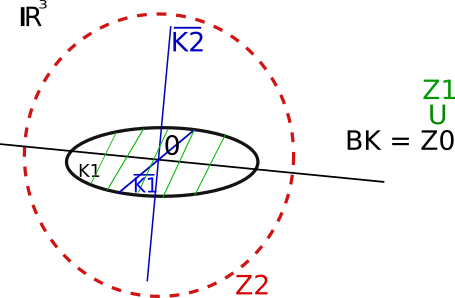
\includegraphics[width=\textwidth]{sphere}
	\end{minipage}} \slide{1in}
	\begin{minipage}[t]{0.4\textwidth}
		$\underset{dim 2}{K_1} \subset \underset{dim 3}{K_3}\n
		\underset{\stackrel{||}{def\B}}{dim K_1} + \underset{\stackrel{||}{dim Im \B}}{dim BK} = 3$
	\end{minipage}\n\n
	$
	\begin{array}{ccl}
		Z_1 & = & BK + K_1 \supset Z_0\\
		\bigcap\\
		Z_2 &= &BK + K_2
	\end{array}\n
	K = \vec{K_1} \oplus \vec{K_2} \oplus BK
	$
	\begin{theorem}
		$0 \leq r \leq m-1\n
		B^r K = B^r \vec K_{r+1} \oplus B^r \vec K_{r+2} \oplus \ldots \oplus B^r \vec K_m \oplus B^{r+1} K$
	\end{theorem}
	\begin{proof}\ \\
		$K = \vec K_1 \oplus \vec K_2 \oplus \ldots \oplus \vec K_m \oplus BK\n
		\forall x \in K \; \; \; x = \underset{\in \vec K_1}{x_1} + \underset{\in \vec K_2}{x_2} + 
		\ldots + \underset{\in \vec K_m}{x_m} + \underset{\in BK}{B x^*}\n
		1\leq r \leq m-1\n
		B^r x = B^r x_1 + B^r x_2 + \ldots + B^r x_r + B^r x_{r+1} + \ldots + B^r x_m + B^{r+1} x^* \boxed{=}\n
		\slide{50pt} B^r x_j = B^{r-j} \underset{\stackrel{||}{\0}}{B^j x_j} = \0\\
		\slide{50pt} 1 \leq j \leq r \; \; \; x_j \in \vec K_j \subseteq K_j = Ker B^j = 
		Ker(\A - \lambda\E)^j|_{K_\lambda}\n
		\boxed{=} B^r x_{r+1} + \ldots + B^r x_m + B^{r+1} x^*$\n
		Дизъюнктность?\n
		$* \; B^r x_{r+1} + B^r x_{r+2} + \ldots + B^r x_m + B^{r+1} x^* = \0\n
		B^r(\underbracket{x_{r+1} + x_{r+2} + \ldots + x_m + Bx^*}_y) = \0\n
		y \in Ker B^r = K_r \subseteq Z_r = \vec K_1 \oplus \ldots \oplus \vec{K_r} \oplus BK\n
		\Rightarrow \underset{\begin{matrix}\text{Однозначно}\\\text{представим}\end{matrix}}{y}
		= x_1 + x_2 + \ldots + x_r + \underset{\mathlarger{x_i \in \vec{K_i}}}Bx^{**}\n
		\slide{1.5cm}||\\
		\underset{\mathlarger{x_{r+i} \in \vec{K_{r+i}}}}{x_{r+1} + x_{r+2} + \ldots + x_m + Bx^*} \Rightarrow \underset{\mathlarger{\forall i = 1\ldots m}}{\boxed{x_i = \0}*}\n
		\Downarrow $ подставим\\
		$\0 + \0 + \ldots + \0 + B^{r+1} x^* = \0 \Rightarrow B^{r+1} x^* = \0 \Rightarrow $ дизъюнктн.
	\end{proof}
	\begin{corollary}
		\ \\
		$K = \uwave{\vec K_1 \oplus \vec K_2 \oplus \ldots \oplus \vec K_m}\oplus 
		\uuline{B\vec K_2 \oplus B \vec K_3 \oplus \ldots \oplus B \vec K_m} \oplus\n
		\oplus \dashuline{B^2 \vec K_3 \oplus  B^2 \vec K_4} \oplus \ldots \oplus 
		B^{m-2} \vec K_{m-1} \oplus B^{m-2} \vec K_m \oplus B^{m-1} \vec K_m$
	\end{corollary}
	\begin{proof}\ \\
		$K = \uwave{\vec K_1 \oplus \vec K_2 \oplus \ldots \oplus \vec K_m} \oplus BK\n
		BK = \uuline{B\vec K_2 \oplus \ldots \oplus B \vec K_m} \oplus B^2 K\n
		B^2 K = \dashuline{B^2 \vec K_3 \oplus B^2 \vec K_4 \oplus \ldots \oplus B^2 \vec K_m} \oplus B^3 K$
	\end{proof}
	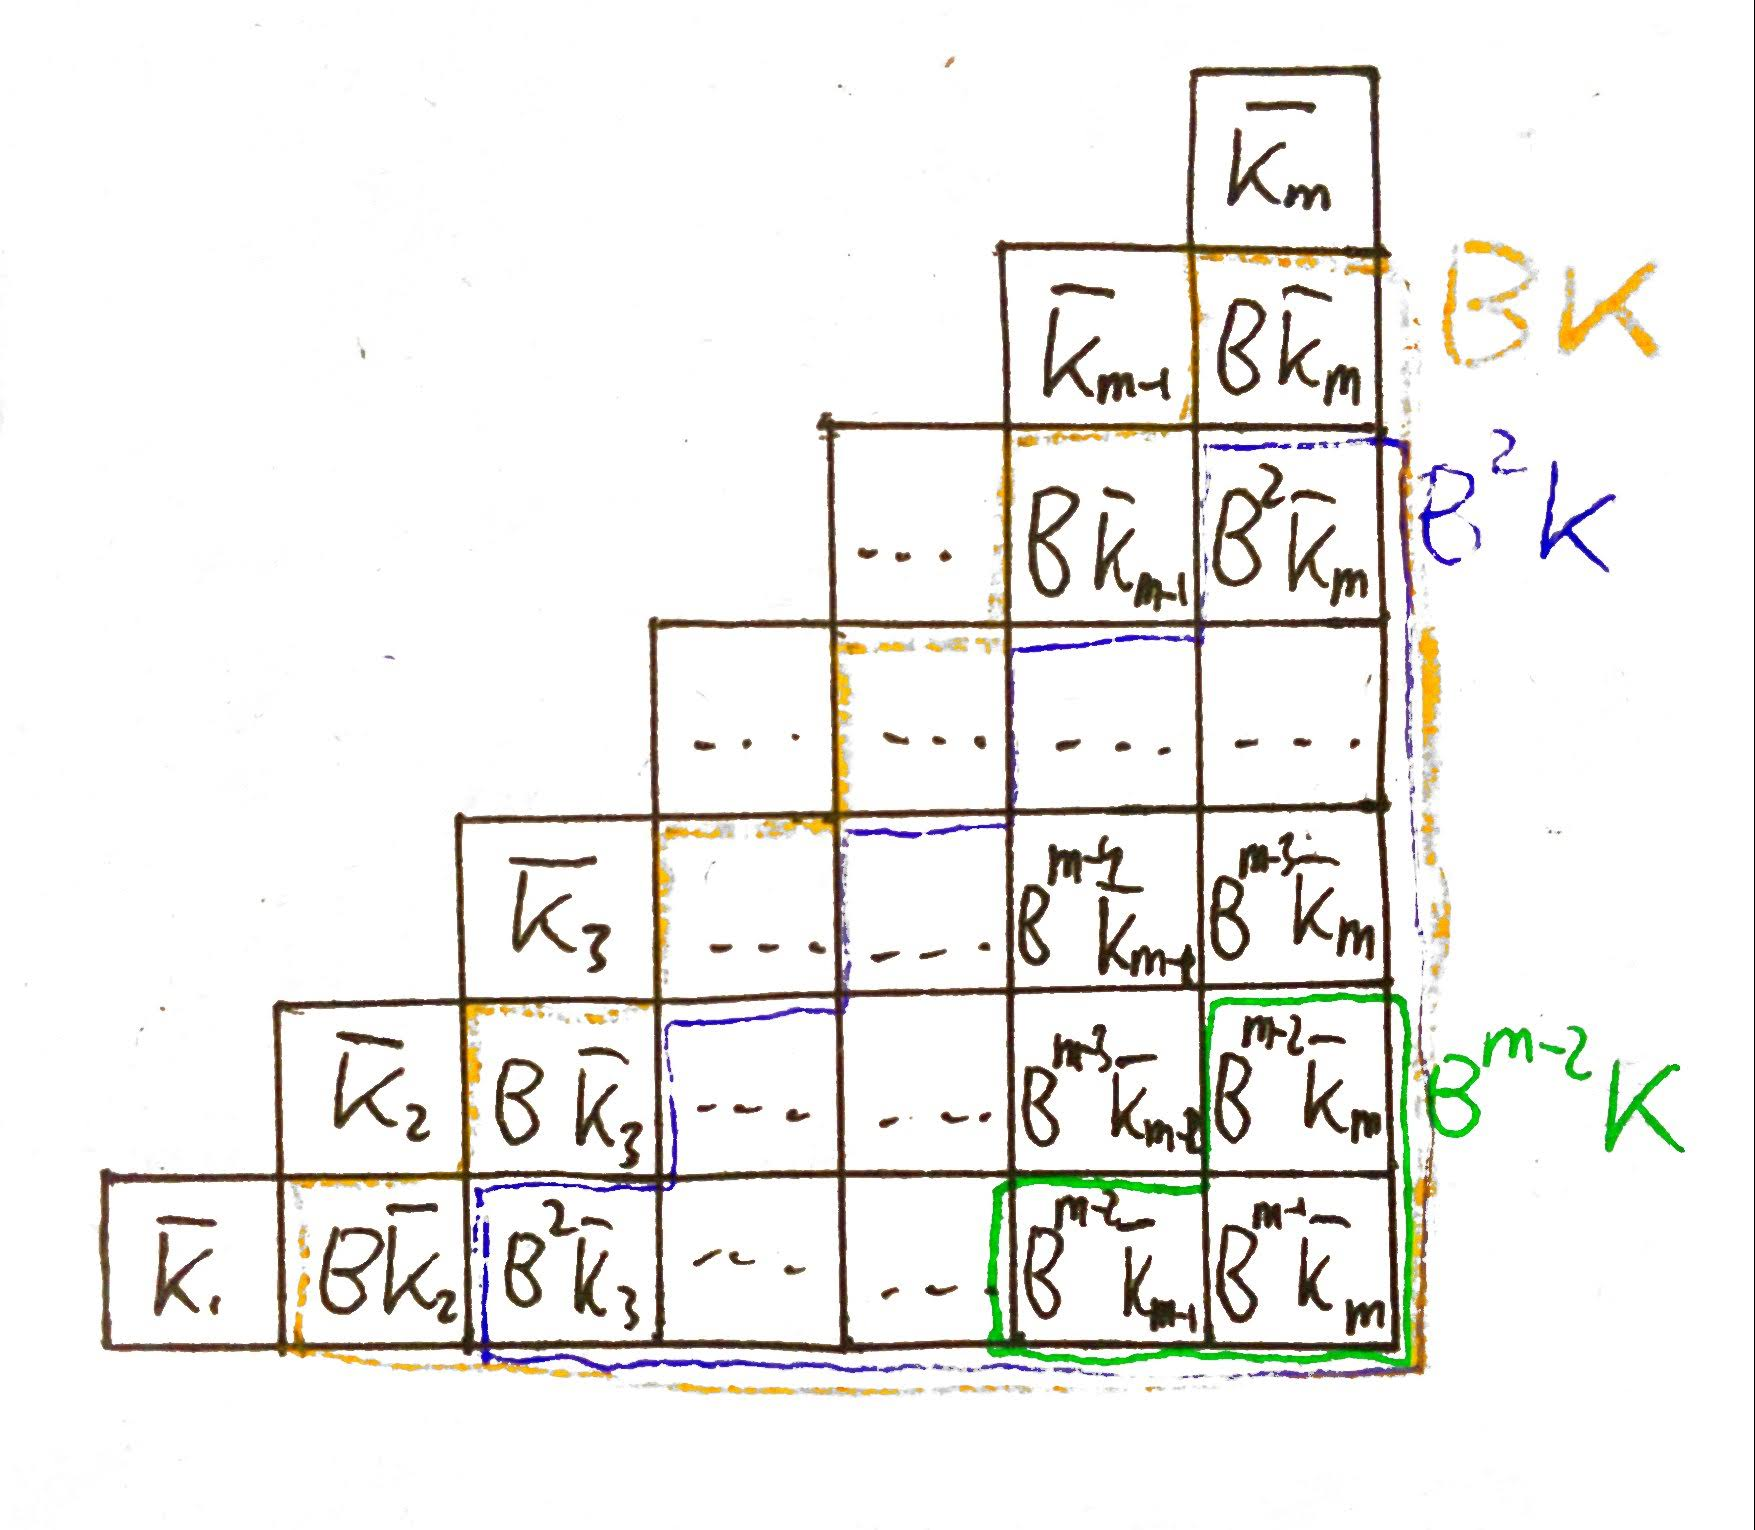
\includegraphics[width=0.7\textwidth]{pyramid}\n
	$\vec K_j$ -- \textbf{Опорные подпространства} \belowbaseline[-12pt]{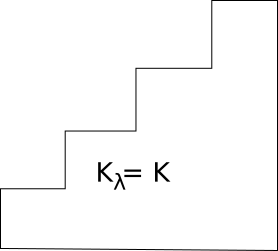
\includegraphics[width=3cm]{sex}}\\
	$1 \leq r \leq m\\
	\text{Если }\vec{K_r} \neq {\0} \longrightarrow \boxed{\tau_r = \vec{K_r} \oplus B\vec{K_r} \oplus
	B^2 \vec{K_r} \oplus \ldots \oplus B^{r-1} \vec{K_r}}$\n
	Башня высоты $r$. "Башня растет вниз"\\
	"Основание"\ башни $\equiv$ опорное подпространство $\vec{K_r}$\\
	"Крыша"\ башни $\equiv B^{r-1} \vec{K_r} \subset V_\lambda\n
	x\in B^{r-1} \vec{K_r} \; \; \quad \begin{matrix}
		x = B^{r-1} y\\
		\underline{y\in \vec{K_r} \subseteq K_r}
	\end{matrix} \;\quad \underline{B x = B^r y = \0}\; \; \; x\in KerB = V_\lambda
	$\n
	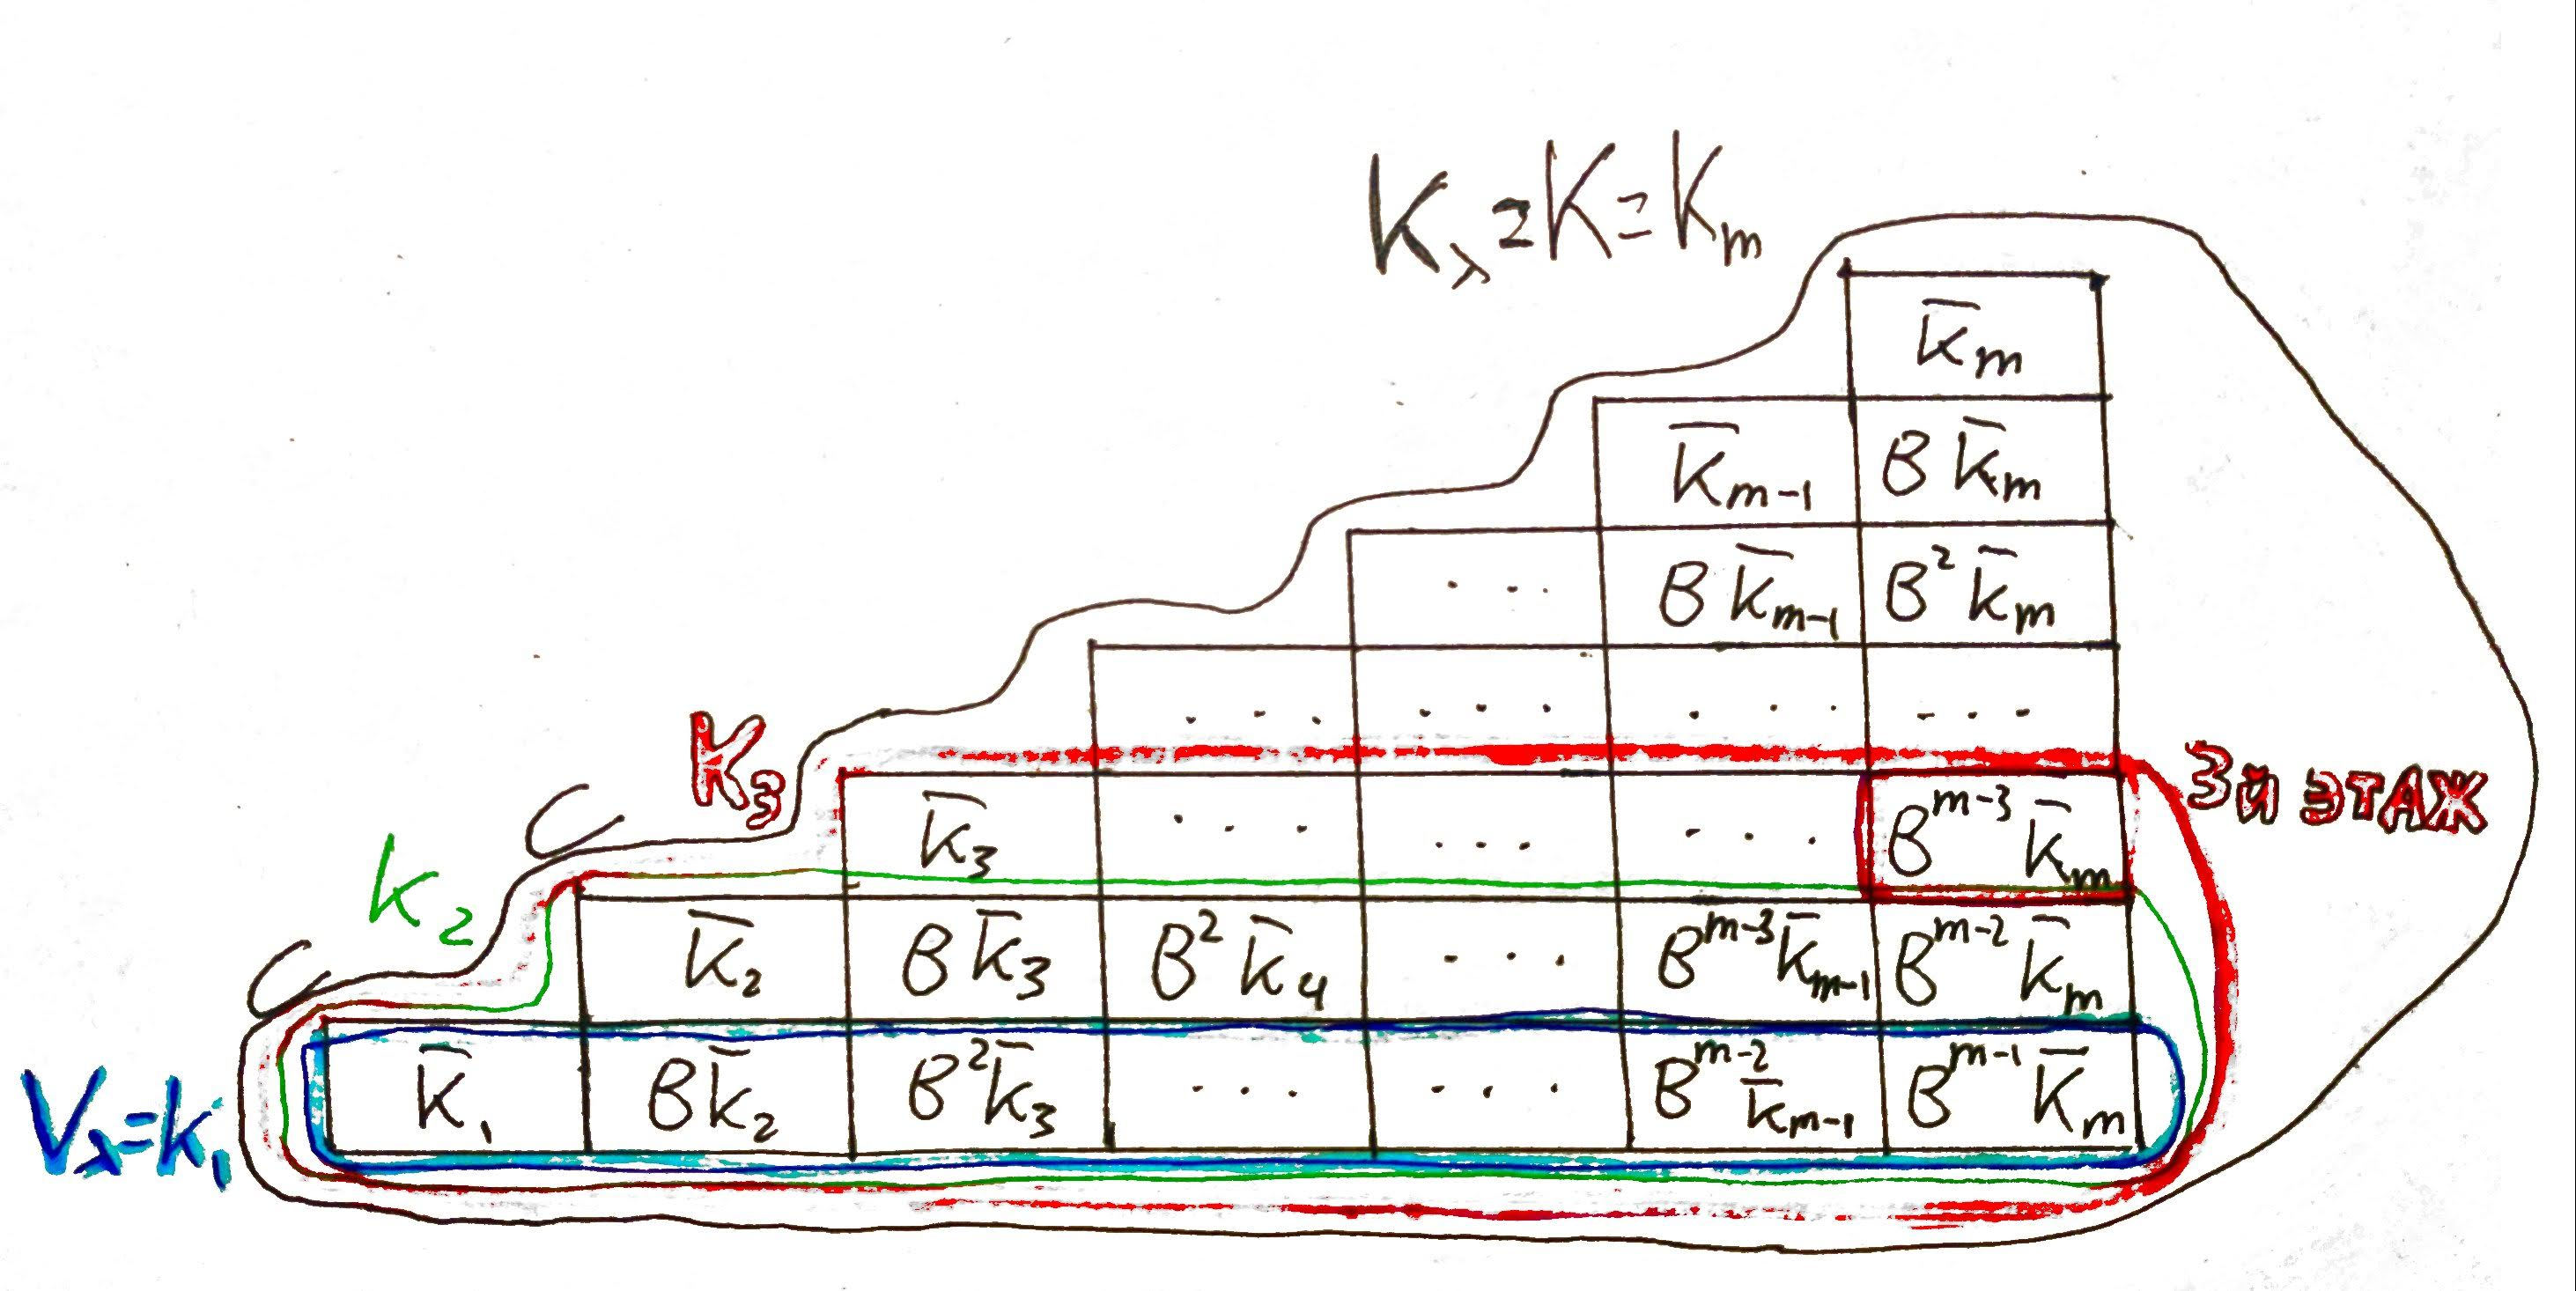
\includegraphics[width=\textwidth]{pyramid2}\n
	Если $K_r = \{\0\}$, то башня высоты $r$ отсутствует. (См. пример, нет башни высоты 2)\n
	$1\leq l \leq m \\
	\vec K_l, B\vec K_{l+1}, B^2 \vec K_{l+2}, \ldots B^{m-1} \vec K_m \; \; \; \; \subset K_l = Ker B^l$\\
	\slide{1in} -- $l$-ые этажи соотв. башен\\
	Покажем: $B^j \vec K_{l+j} \subset K_l\n
	B^l(B^j \vec K_{l+j}) = (B^{l+ j}) \underset{ \subset K_{l+j} = Ker B^{l+j}}{\vec K_{l+ j}} = \0 \Rightarrow
	B^j \vec K_{l+j} \subset K_l\n
	K = \bigoplus\limits_{r=1}^m \tau_r$
	\begin{theorem}[О размерности башни]\ \\
		$\forall \tau_r$ любой этаж башни имеет одну и ту же размерность $d_r = dim \vec K_r = $ ширина башни.\n
		$\begin{array}{cc}
			r \text{ высота } \updownarrow & 
			\begin{array}{|c|}
				\cline{1-1}
				\vec K_r\\
				\cline{1-1}
				B\vec K_r\\
				\cline{1-1}
				B^2 \vec K_r\\
				\cline{1-1}
				\ldots\\
				\cline{1-1}
				B^{r-1} \vec K_r\\
				\cline{1-1}
				\multicolumn{1}{c}{\tau_r}
			\end{array}
		\end{array} \quad \quad \boxed{d_r = dim \vec K_r} = $ ширина башни
	\end{theorem}
	\begin{proof}
		\ \\
		$B^j|_{\vec K_r}: \vec K_r \rightarrow B^j \vec K_r\n
		B^j_{\vec K_r}$ изоморфизм "?"\n
		$Ker B^j|_{\vec K_r} = \{\0\}$ тривиально "?"\n
		\belowbaseline[-12pt]{$\begin{array}{l}
			x\in \vec K_r \subset K_r \subset Z_r \\
			\underset{j = 1\ldots r-1}{x \in Ker B^j = K_j \rightarrow}
		\end{array}$}
		$\underset{\nearrow}{=}$
		\belowbaseline[-12pt]{$
			\begin{array}{c}
				Z_{r-1}\\
				\cup\\
				K_{r-1}\\
				\cup\\
				\vdots\\
				\cup\\
				K_1
			\end{array}
		$} $\oplus \overset{\mathlarger{\stackrel{\ni x}{\downarrow}}}{\vec K_r}
		\Rightarrow \boxed{x = \0} \quad \quad \boxed{Z_{r-1} = BK + K_{r-1}}\n
		\Rightarrow $ Изоморфизм $\Rightarrow dim(\vec{K_r}) = dim(B^j \vec K_r) = d_r$
	\end{proof}
	\begin{corollary}
		$\sum\limits_{r=1}^m d_r = dim V_\lambda = \gamma(\lambda)\n
		\sum\limits_{r=1}^m \underbracket{r\cdot d_r}_{dim \ \tau_r} = dim K_\lambda = dim K = \alpha(\lambda)$
	\end{corollary}
	\begin{corollary}[Теорема Фробениуса]
		\ \\
		$d_r = rg B^{r-1} - 2rg B^r + rg B^{r+1}\n
		(d_m = rg B^{r-1})$
	\end{corollary}
	\begin{proof} \ \\
		$B^r K = B^r \vec K_{r+1} \oplus B^r \vec K_{r+2} \oplus \ldots \oplus B^r \vec K_m \oplus B^{r+1} K\n
		\rho:= rg B^r = d_{r+1} + d_{r+2} + \ldots + d_m + \underbracket{rg B^{r+1}}_{\rho_{r+1}}
		$
		\begin{align*}
			d_1 + d_2 + \ldots + d_m &= \rho_0 - \rho_1 \\
			d_2 + \ldots + d_m &= \rho_1 - \rho_2 & \downarrow-\\
			d_3 + \ldots + d_m &= \rho_2 - \rho_3& \downarrow-\\
			d_{m-2} + d_{m-1} + d_m &= \rho_{m-3} - \rho_{m-2}& \downarrow-\\
			d_{m-1} + d_m &= \rho_{m-2} - \rho_{m-1} & \downarrow-\\
			d_m &= \rho_{m-1} & \downarrow-\\
			& \rho_m = 0
		\end{align*}
		$\boxed{d_r = \rho_{r-1} - 2\rho_r + \rho_{r+1}}$
	\end{proof}
\end{document}